\section{Voice}

Voice is the most common feature describing the predicate. It describes the relationship between the action the predicate expresses and the participants of the action (the subject, objects etc.).

There are three voices in Novoslovnica:

\begin{itemize}
	\item Active
	\item Middle
	\item Passive
\end{itemize}

\begin{figure}
	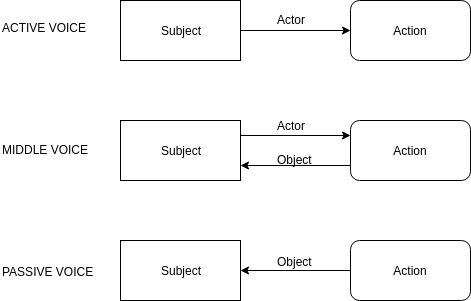
\includegraphics[width=\linewidth]{./sources/voices.png}
	\caption{Voices in Novoslovnica}
	\label{fig:voices}
\end{figure}

\textbf{Active voice}


\textbf{Middle voice}

\textbf{Passive voice}
